\hspace{24pt}
\renewcommand{\baselinestretch}{1.5}
\newcommand{\subSCPT}[1]{\hspace{0.08em}\textsubscript{#1}}
\newcommand{\stratified}{\subSCPT{stratified}}

In this chapter, we will explain our experiments in detail. First, we describe the experimental environment in Section~\ref{environment}. Second, we introduce the dataset from ENCODE, the method used to select from many datasets in Section~\ref{dataset}. Third, before showing the performance, we depict evaluation metrics in Section~\ref{metric}. Fourth, we show experiment results from different models to compare their performance in Section~\ref{performance}. Finally, we further analyze our model by visualization of feature vectors in Section~\ref{discuss}.

\section{Environment} \label{environment}
We use PyTorch, one of the most popular deep learning libraries \cite{paszke2017automatic}, to construct the architecture of our model.  PyTorch can be trained and operated on a CUDA-capable Nvidia GPU to increase computational speed.  Our GPU is GEFORCE RTX 2070 SUPER. In order to more conveniently monitor the model, we use Weights \& Biases (wandb) \cite{wandb} for logging hyper-parameters and output metrics, then quickly visualize and compare results with dashboard on website.

\section{Dataset} \label{dataset}
We download datasets from the ENCODE project. This project is being conducted by the ENCODE consortium, funded by the National Human Genome Research Institute. The goal of ENCODE is to build a comprehensive list of functional elements in the human genome. To ensure high quality of analysis, ENCODE investigators employ a variety of assays and methods to identify various functional elements, and all generated data is available on ENCODE website \cite{davis2018encyclopedia}.

We selected three cell lines as datasets, including A549, GM12878 and K562. However, each type of epigenetic data on the ENCODE website may be measured by different laboratories, while setting the different parameters in conducting experiments may influence the observed data. Hence, we select our datasets according to the warnings represented on ENCODE website. These warnings may indicate an error in the experimental metadata, or may indicate that the data itself does not meet some aspect of the consortium’s standards. There are three flag’s colors corresponding to the severity of the problem \cite{davis2018encyclopedia}.

\begin{figure}[H]
    \centering
    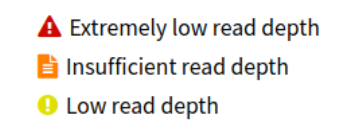
\includegraphics[width=0.5\columnwidth]{body/figure/figure13.png}
    \captionsetup{labelfont=bf}
    \renewcommand{\baselinestretch}{1.0}
    \caption[Example of warning levels]{This figure is a screenshot from the ENCODE website. The example shows that different levels of severity in low read depth, which acts as metric to evaluate the quality of sequencing experiment.}
    \label{f13}
\end{figure}

Therefore, we chose our datasets based on the number and severity of any associated warnings.

\section{Evaluation Metrics} \label{metric}
We use two metrics to evaluate our model. There are respectively area under the receiver operating characteristics curve (ROC) and area under the precision-recall curve (PRC). These metrics are common evaluations of a classifier’s prediction performance, which are threshold-free measures.

Before introducing area under ROC and area under PRC, we first introduce the confusion matrix because these metrics are composed of the elements of this matrix. The confusion matrix consists of true positive (TP), false positive (FP), true negative (TN) and false negative (FN), as shown in Figure~\ref{f14}. Each row of the matrix represents the instances in an actual class while each column represents the instances in a predicted class, or vice versa. The several basic metrics are calculated by elements of confusion matrix, including precision, recall (also called sensitivity) and specificity \cite{saito2015precision}, shown in the box below.

\begin{center}
\fcolorbox{black}{gray!10}{
\begin{tabular}{ll}
Precision:            &  $\frac{\text{TP}}{\text{TP+FP}}$\\
Recall(sensitivity):  &  $\frac{\text{TP}}{\text{TP+FN}}$\\
Specificity:          &  $\frac{\text{TN}}{\text{TN+FP}}$
\end{tabular}
}
\end{center}



\begin{figure}[H]
    \centering
    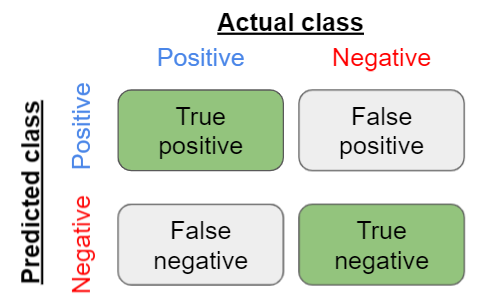
\includegraphics[width=0.65\columnwidth]{body/figure/figure14.png}
    \captionsetup{labelfont=bf}
    % \renewcommand{\baselinestretch}{1.0}
    \caption[Confusion matrix]{Confusion matrix.}
    \label{f14}
\end{figure}

Then, ROC is plotted by sensitivity and specificity, and PRC is plotted by precision and recall. Areas under these curves are metrics used in evaluating our model. In addition, these curves provide useful information of baseline (random classifier). The baseline showed in ROC is a diagonal line, whereas the baseline showed in PRC is determined by the ratio of positives (P) and negatives (N) as y = P / (P+N) \cite{saito2015precision}, shown in Figure~\ref{f15}.

\begin{figure}[H]
    \centering
    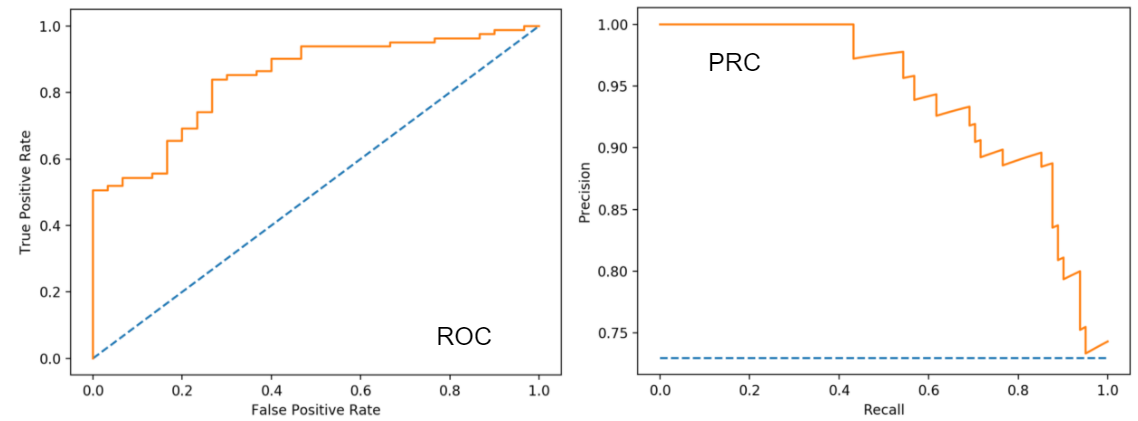
\includegraphics[width=1\columnwidth]{body/figure/figure15.png}
    \vspace{-1cm}
    \captionsetup{labelfont=bf}
    \renewcommand{\baselinestretch}{1.0}
    \caption[ROC and PRC]{Solid line represents monitored model. Dotted line represents baseline (random classifier). And, area under these curves represents performance of these models. (figure reproduced from \cite{rocprc})}
    \label{f15}
\end{figure}

\section{Prediction Performance} \label{performance}
In order to evaluate whether introducing techniques and features are helpful to our model, we designed a series of experiments.  In the following we describe these experiments and show the results. Finally, we will show the results of best model trained on all cell lines in Section~\ref{cross}.

\subsection{Baseline}
We construct a CNN according to the architecture of DeepSEA \cite{zhou2015predicting}, which acts as a baseline. The baseline is depicted in Figure~\ref{f16}, and is trained with the same training methodology as our model, described in Section~\ref{method}. Only difference is the number of neurons in the last fully connected layer. We focus on data imputation of six histone modifications, instead of interaction of various chromatin states. Therefore, we change the amount of neurons in the last fully connected layer to six.

\begin{figure}[H]
    \centering
    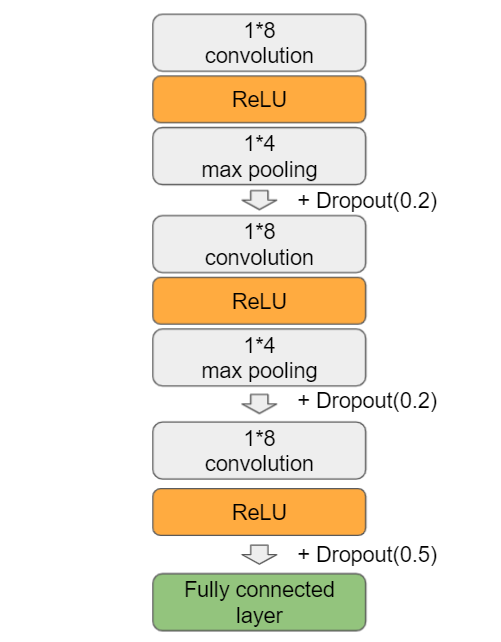
\includegraphics[width=0.6\columnwidth]{body/figure/figure16.png}
    \captionsetup{labelfont=bf}
    \renewcommand{\baselinestretch}{1.0}
    \caption[Framework of baseline]{The framework of our baseline is same with DeepSEA.}
    \label{f16}
\end{figure}

\subsection{Inception Module}
For experimental efficiency, we first select nine partitions (1369713 windows) of K562 to train the baseline and our model, and then evaluate on one partition (152191 windows) of K562 to compare the results of these models.  As mentioned Section~\ref{metric}, we use area under ROC (AUROC) and area under PRC (AUPRC) as evaluation metrics.

Here, we want to observe the change of results after adding an inception module into our model. Our model is named “Inception” in the following tables. Apparently, we improve the prediction in all cases compared to baseline, shown in Table~\ref{t4} and Table~\ref{t5}.

\subsection{Stratified Mini-batch} \label{strat}
According to same settings with above experiment, we want to test whether stratified mini-batch is good for our task, that is imbalanced multi-label classification, shown in Table~\ref{t4} and Table~\ref{t5}. In the following tables, we use subscript to represent the model adding stratified mini-batch. In addition, we test on not only our model but also baseline, in order to check whether this mechanism only helps on special case.

\begin{table}[H]%加入table環境指令以控制表格的位置、編號與標題,[h]代表將表格置於here,其他位置的標示請參考手冊
    \centering
    \begin{tabular}{lcccc}
    \hline
    Model & Baseline & Baseline\stratified & Inception & Inception\stratified \\\hline
    H3K4me3 & 0.979 & 0.9819 & 0.9902 & \textbf{0.9927} \\
    H3K27ac & 0.9278 & 0.9334 & 0.9488 & \textbf{0.9549} \\
    H3K4me1 & 0.9672 & 0.9718 & 0.9745 & \textbf{0.9787} \\
    H3K36me3 & 0.985 & 0.9854 & 0.9857 & \textbf{0.9886} \\
    H3K9me3 & 0.9283 & 0.9429 & 0.9726 & \textbf{0.9762} \\
    H3K27me3 & 0.9923 & 0.9938 & 0.9964 & \textbf{0.9969} \\\hline
    \end{tabular}
    \captionsetup{labelfont=bf}
    \renewcommand{\baselinestretch}{1.0}
    \caption[Comparison of baseline and inception with AUROC]{This table represents performance with AUROC. Best predictive performance of each histone modification is shown in bold.}
    \label{t4}
\end{table}

\begin{table}[H]%加入table環境指令以控制表格的位置、編號與標題,[h]代表將表格置於here,其他位置的標示請參考手冊
    \centering
    \begin{tabular}{lcccc}
    \hline
    Model & Baseline & Baseline\stratified & Inception & Inception\stratified \\\hline
    H3K4me3 & 0.8995 & 0.9089 & 0.9365 & \textbf{0.9474} \\
    H3K27ac & 0.723 & 0.7385 & 0.7754 & \textbf{0.7934} \\
    H3K4me1 & 0.9388 & 0.9465 & 0.9501 & \textbf{0.9588} \\
    H3K36me3 & 0.8886 & 0.8905 & 0.9082 & \textbf{0.9208} \\
    H3K9me3 & 0.541 & 0.5911 & 0.7641 & \textbf{0.8114} \\
    H3K27me3 & 0.9905 & 0.9925 & 0.996 & \textbf{0.9965} \\\hline
    \end{tabular}
    \captionsetup{labelfont=bf}
    \renewcommand{\baselinestretch}{1.0}
    \caption[Comparison of baseline and inception with AUPRC]{This table represents performance with AUPRC. Best predictive performance of each histone modification is shown in bold.}
    \label{t5}
\end{table}

Regardless of the frameworks in above table, adding the inception model and stratified mini-batch mechanism outperforms the original model.  And the model which introduces inception module and stratified mini-batch obtains the best results in above experiments. Hence, we decide to use this model to extract features from DNA sequences and DNA methylation signal, and then use these features to predict histone modifications.

\subsection{DNA methylation}
After confirming these techniques are helpful, we wanted to observe how much different input features influence the results of the model. We separately extract features from only DNA sequence, only DNA methylation signal and both, as well as represent them by subscripts in the following tables.  As in the above experiments, all models are trained on the K562 cell line. In addition, we further check whether the framework of DeepSEA can also improve prediction by adding features from DNA methylation signal, as shown in Tables \ref{t6}, \ref{t7}, \ref{t8}, and \ref{t9}.


\newcommand*{\explainUnderlinesAndBold}{For each histone modification, the best single source (Meth or DNA) performance is underlined and the best overall performance is shown in bold}

\begin{table}[H]%加入table環境指令以控制表格的位置、編號與標題,[h]代表將表格置於here,其他位置的標示請參考手冊
    \centering
    \begin{tabular}{lccc}
    \hline
    Model & Baseline\subSCPT{Meth} & Baseline\subSCPT{DNA} & Baseline\subSCPT{DNA+Meth} \\\hline
    H3K4me3 & 0.8963 & \underline{0.9741} & \textbf{0.9819} \\
    H3K27ac & 0.8475 & \underline{0.9172} & \textbf{0.9334} \\
    H3K4me1 & \underline{0.9435} & 0.8943 & \textbf{0.9718} \\
    H3K36me3 & \underline{0.9766} & 0.8982 & \textbf{0.9854} \\
    H3K9me3 & 0.7912 & \textbf{\underline{0.9468}} & 0.9429 \\
    H3K27me3 & \underline{0.9612} & 0.9287 & \textbf{0.9938} \\\hline
    \end{tabular}
    \captionsetup{labelfont=bf}
    \renewcommand{\baselinestretch}{1.0}
    \caption[Comparison of different inputs of baseline with AUROC]{This table represents performance with AUROC. \explainUnderlinesAndBold.}
    \label{t6}
\end{table}

\begin{table}[H]%加入table環境指令以控制表格的位置、編號與標題,[h]代表將表格置於here,其他位置的標示請參考手冊
    \centering
    \begin{tabular}{lccc}
    \hline
    Model & Baseline\subSCPT{Meth} & Baseline\subSCPT{DNA} & Baseline\subSCPT{DNA+Meth} \\\hline
    H3K4me3 & 0.6433 & \underline{0.8562} & \textbf{0.9089} \\
    H3K27ac & 0.5413 & \underline{0.6928} & \textbf{0.7385} \\
    H3K4me1 & \underline{0.8942} & 0.8183 & \textbf{0.9465} \\
    H3K36me3 & \underline{0.8404} & 0.5417 & \textbf{0.8905} \\
    H3K9me3 & 0.1271 & \underline{0.5883} & \textbf{0.5911} \\
    H3K27me3 & \underline{0.9429} & 0.9197 & \textbf{0.9925} \\\hline
    \end{tabular}
    \captionsetup{labelfont=bf}
    \renewcommand{\baselinestretch}{1.0}
    \caption[Comparison of different inputs of baseline with AUPRC]{This table represents performance with AUPRC. \explainUnderlinesAndBold.}
    \label{t7}
\end{table}

\begin{table}[H]%加入table環境指令以控制表格的位置、編號與標題,[h]代表將表格置於here,其他位置的標示請參考手冊
    \centering
    \begin{tabular}{lccc}
    \hline
    Model & Inception\subSCPT{Meth} & Inception\subSCPT{DNA} & Inception\subSCPT{DNA+Meth} \\\hline
    H3K4me3 & 0.9204 & \underline{0.9806} & \textbf{0.9927} \\
    H3K27ac & 0.8719 & \underline{0.93} & \textbf{0.9549} \\
    H3K4me1 & \underline{0.9481} & 0.9144 & \textbf{0.9787} \\
    H3K36me3 & \underline{0.9789} & 0.9119 & \textbf{0.9886} \\
    H3K9me3 & 0.8198 & \underline{0.9648} & \textbf{0.9762} \\
    H3K27me3 & \underline{0.9705} & 0.9532 & \textbf{0.9969} \\\hline
    \end{tabular}
    \captionsetup{labelfont=bf}
    \renewcommand{\baselinestretch}{1.0}
    \caption[Comparison of different inputs of inception with AUROC]{This table represents performance with AUROC. \explainUnderlinesAndBold.}
    \label{t8}
\end{table}

\begin{table}[H]%加入table環境指令以控制表格的位置、編號與標題,[h]代表將表格置於here,其他位置的標示請參考手冊
    \centering
    \begin{tabular}{lccc}
    \hline
    Model & Inception\subSCPT{Meth} & Inception\subSCPT{DNA} & Inception\subSCPT{DNA+Meth} \\\hline
    H3K4me3 & 0.6971 & \underline{0.8775} & \textbf{0.9474} \\
    H3K27ac & 0.5741 & \underline{0.7134} & \textbf{0.7934} \\
    H3K4me1 & \underline{0.9033} & 0.8514 & \textbf{0.9588} \\
    H3K36me3 & \underline{0.852} & 0.6141 & \textbf{0.9208} \\
    H3K9me3 & 0.1585 & \underline{0.6936} & \textbf{0.8114} \\
    H3K27me3 & \underline{0.96} & 0.9507 & \textbf{0.9965} \\\hline
    \end{tabular}
    \captionsetup{labelfont=bf}
    \renewcommand{\baselinestretch}{1.0}
    \caption[Comparison of different inputs of inception with AUPRC]{This table represents performance with AUPRC. \explainUnderlinesAndBold.}
    \label{t9}
\end{table}

It is obvious that models, which input DNA sequences and methylation signal, obtain better performance than models, which only extract features from DNA sequence.  Interestingly, the models predicting H3K4me1, H3K36me3 and H3K27me3 only input the features from DNA methylation signal yields better results than the model using only DNA sequence. Therefore, DNA methylation provide more information for the models and improves prediction.

\subsection{Cross cell lines} \label{cross}
According to a series of experiments, we confirm that introducing certain techniques and features are good for our model.
Next, we trained Inception\subSCPT{DNA+Meth} on different cell lines, including A549, GM12878 and K562, to get more information across cell lines. Similarly, we selected nine partitions of each cell line to train, and evaluated on one partition of each cell line. Number of data points for training and testing separately are 4760181 and 528909. We show the mean of performance in the Table~\ref{t10} and Table~\ref{t11}.

\begin{table}[H]%加入table環境指令以控制表格的位置、編號與標題,[h]代表將表格置於here,其他位置的標示請參考手冊
    \centering
    \begin{tabular}{lccc}
    \hline
    Model & Inception\subSCPT{Meth} & Inception\subSCPT{DNA} & Inception\subSCPT{DNA+Meth} \\\hline
    H3K4me3 & 0.9214 & \underline{0.9657} & \textbf{0.984} \\
    H3K27ac & 0.8422 & \underline{0.8659} & \textbf{0.9288} \\
    H3K4me1 & \underline{0.8772} & 0.8511 & \textbf{0.9441} \\
    H3K36me3 & \underline{0.9576} & 0.8998 & \textbf{0.9774} \\
    H3K9me3 & 0.8018 & \underline{0.9518} & \textbf{0.9719} \\
    H3K27me3 & \underline{0.9557} & 0.909 & \textbf{0.9915} \\\hline
    \end{tabular}
    \captionsetup{labelfont=bf}
    \renewcommand{\baselinestretch}{1.0}
    \caption[Comparison of different inputs across cell lines with AUROC]{This table represents performance with AUROC. \explainUnderlinesAndBold.}
    \label{t10}
\end{table}

\begin{table}[H]%加入table環境指令以控制表格的位置、編號與標題,[h]代表將表格置於here,其他位置的標示請參考手冊
    \centering
    \begin{tabular}{lccc}
    \hline
    Model & Inception\subSCPT{Meth} & Inception\subSCPT{DNA} & Inception\subSCPT{DNA+Meth} \\\hline
    H3K4me3 & 0.6863 & \underline{0.83} & \textbf{0.9006} \\
    H3K27ac & 0.6231 & \underline{0.6662} & \textbf{0.7862} \\
    H3K4me1 & \underline{0.7223} & 0.6694 & \textbf{0.8565} \\
    H3K36me3 & \underline{0.8803} & 0.7859 & \textbf{0.9415} \\
    H3K9me3 & 0.2386 & \underline{0.6865} & \textbf{0.7987} \\
    H3K27me3 & \underline{0.8995} & 0.8497 & \textbf{0.9834} \\\hline
    \end{tabular}
    \captionsetup{labelfont=bf}
    \renewcommand{\baselinestretch}{1.0}
    \caption[Comparison of different inputs across cell lines with AUPRC]{This table represents performance with AUPRC. \explainUnderlinesAndBold.}
    \label{t11}
\end{table}

\section{Discussion} \label{discuss}
Furthermore, we want to examine whether our model learned relationships which generalize across cell lines, by visualizing representation of each data point, called feature vector, that is input of fully connected layers in our model. First, we use the method of dimension reduction, t-distributed stochastic neighbor embedding (t-SNE), to covert each feature vector to two dimensions and three dimensions. Next, we utilize scatter plot to observe distribution of converted vector in each cell line through plotting different colors to annotate which cell line is it.

In order to observe which input feature provide the most information of crossing cell lines, we individually visualize the feature vectors generated by models, which models are trained according to previous experiment in Section~\ref{cross}.

\begin{figure}[H]
    \centering
    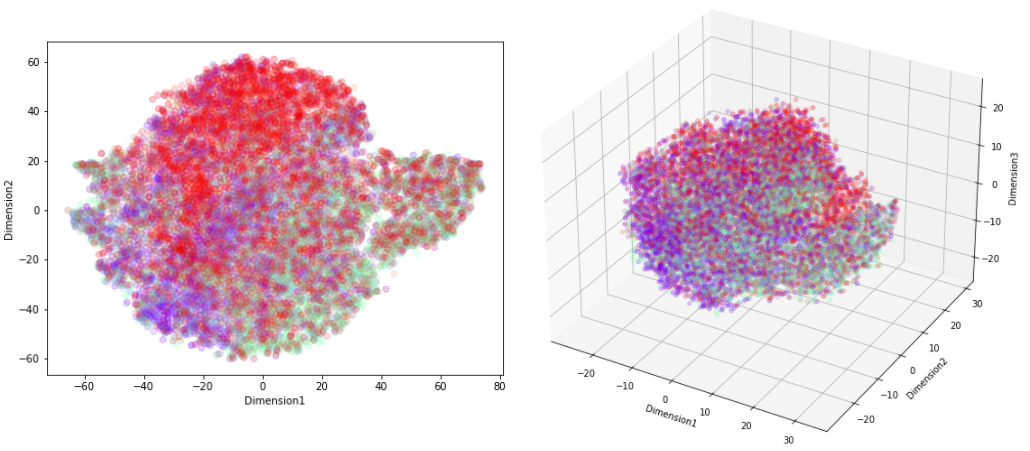
\includegraphics[width=1\columnwidth]{body/figure/figure17.png}
    \captionsetup{labelfont=bf}
    \renewcommand{\baselinestretch}{1.0}
    \caption[Visualization of feature vectors generated by Inception\subSCPT{DNA}]{Visualization of feature vectors generated by Inception\subSCPT{DNA}.}
    \label{f17}
\end{figure}

\begin{figure}[H]
    \centering
    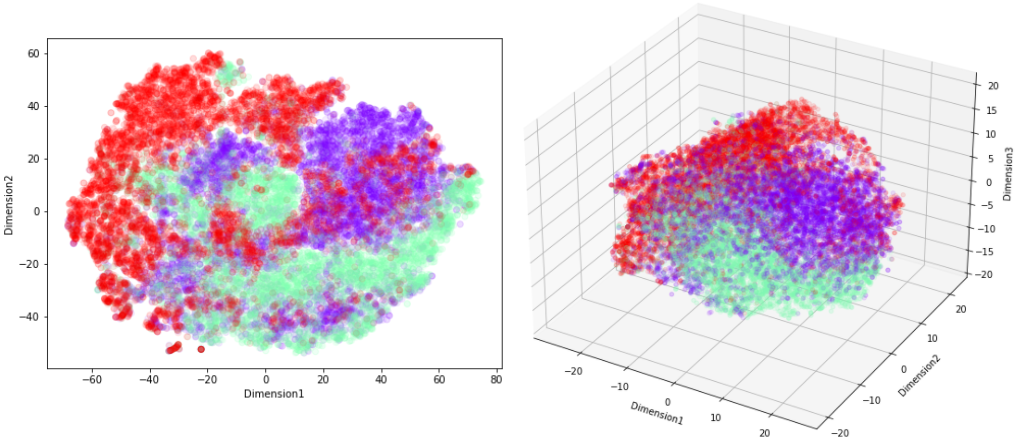
\includegraphics[width=1\columnwidth]{body/figure/figure18.png}
    \captionsetup{labelfont=bf}
    \renewcommand{\baselinestretch}{1.0}
    \caption[Visualization of feature vectors generated by Inception\subSCPT{Meth}]{Visualization of feature vectors generated by Inception\subSCPT{Meth}.}
    \label{f18}
\end{figure}

\begin{figure}[H]
    \centering
    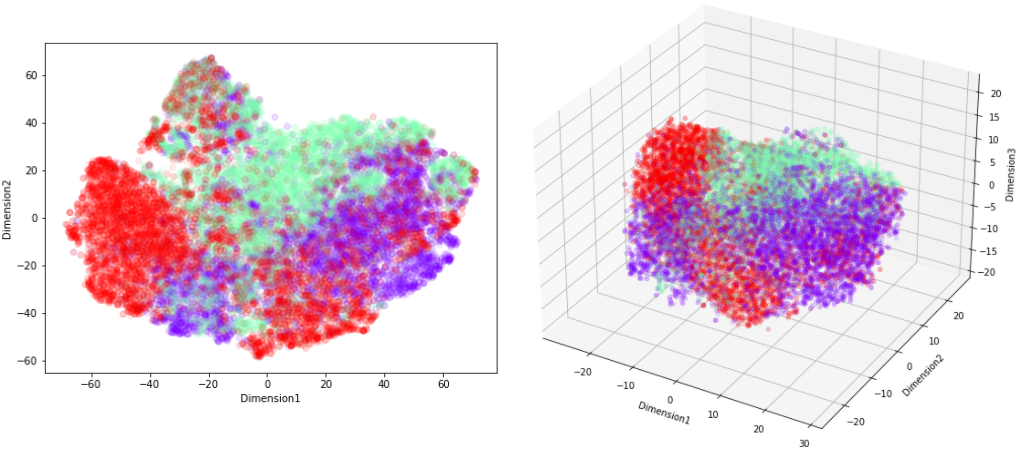
\includegraphics[width=1\columnwidth]{body/figure/figure19.png}
    \captionsetup{labelfont=bf}
    \renewcommand{\baselinestretch}{1.0}
    \caption[Visualization of feature vectors generated by Inception\subSCPT{DNA+Meth}]{Visualization of feature vectors generated by Inception\subSCPT{DNA+Meth}.}
    \label{f19}
\end{figure}

By above visualization, we clearly observe variations of distribution. As long as adding input feature of DNA methylation, the model will learn cell line-specific information via DNA methylation, and automatically discriminate different biosamples within whole feature vectors. This phenomenon is not observed with the model only using input features of DNA sequences.
